\documentclass[crop,tikz,ifthenelse]{standalone}
\usetikzlibrary{calc}
\begin{document}
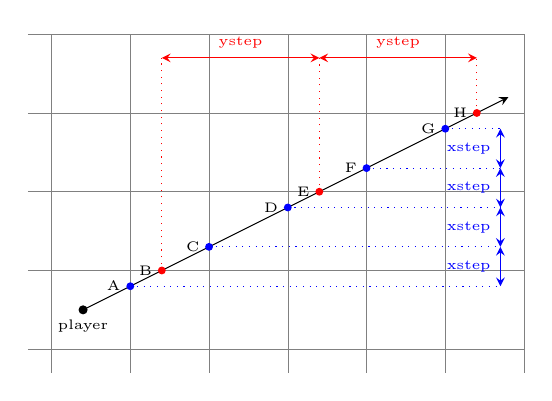
\begin{tikzpicture}[]

\newcommand\minx{-0.3}
\newcommand\maxx{6}

\newcommand\miny{-0.3}
\newcommand\maxy{4}

\draw[step=1,gray,very thin] (\minx,\miny) grid (\maxx, \maxy);


\coordinate(player) at (0.4,0.5);
\fill[draw=black] (player) circle (0.05)  node[align=center, below] {\tiny player};

\coordinate(endray) at (5.8, 3.2);

\draw[->, >=stealth] (player) -- (endray);

%\coordinate (A) at (intersection of player--endray and {1,-1}--{1,4}) ; 
%node[align=center, above] {\tiny A};
%\draw (A) circle (0.05)   

\coordinate(line1_p1) at (1,\miny) {};
\coordinate(line1_p2) at (1,\maxy) {};
\coordinate (A) at (intersection of player--endray and line1_p1--line1_p2);
\node[align=center, left] at (A) {\tiny A};
\fill[blue] (A) circle (0.05);

\coordinate(hline1_p1) at (\minx,1) {};
\coordinate(hline1_p2) at (\maxx,1) {};
\coordinate (B) at (intersection of player--endray and hline1_p1--hline1_p2);
\node[align=center, left] at (B) {\tiny B};
\fill[red] (B) circle (0.05);

\coordinate(line2_p1) at (2,\miny) {};
\coordinate(line2_p2) at (2,\maxy) {};
\coordinate (C) at (intersection of player--endray and line2_p1--line2_p2);
\node[align=center, left] at (C) {\tiny C};
\fill[blue] (C) circle (0.05);


\coordinate(line3_p1) at (3,-1) {};
\coordinate(line3_p2) at (3,4) {};
\coordinate (D) at (intersection of player--endray and line3_p1--line3_p2);
\node[align=center, left] at (D) {\tiny D};
\fill[blue] (D) circle (0.05);

\coordinate(hline2_p1) at (-1,2) {};
\coordinate(hline2_p2) at (5,2) {};
\coordinate (E) at (intersection of player--endray and hline2_p1--hline2_p2);
\node[align=center, left] at (E) {\tiny E};
\fill[red] (E) circle (0.05);

\coordinate(line4_p1) at (4,-1) {};
\coordinate(line4_p2) at (4,4) {};
\coordinate (F) at (intersection of player--endray and line4_p1--line4_p2);
\node[align=center, left] at (F) {\tiny F};
\fill[blue] (F) circle (0.05);

\coordinate(line5_p1) at (5,-1) {};
\coordinate(line5_p2) at (5,4) {};
\coordinate (G) at (intersection of player--endray and line5_p1--line5_p2);
\node[align=center, left] at (G) {\tiny G};
\fill[blue] (G) circle (0.05);


\coordinate(hline3_p1) at (-1,3) {};
\coordinate(hline3_p2) at (5,3) {};
\coordinate (H) at (intersection of player--endray and hline3_p1--hline3_p2);
\node[align=center, left] at (H) {\tiny H};
\fill[red] (H) circle (0.05);

\newcommand\xprojection{5.7}
%\fill[blue] ($(\xprojection, -1)!(A)!(\xprojection, 5)$) circle (0.05); 
%\fill[blue] ($(\xprojection, -1)!(C)!(\xprojection, 5)$) circle (0.05);
%\fill[blue] ($(\xprojection, -1)!(D)!(\xprojection, 5)$) circle (0.05);
%\fill[blue] ($(\xprojection, -1)!(F)!(\xprojection, 5)$) circle (0.05);
%\fill[blue] ($(\xprojection, -1)!(G)!(\xprojection, 5)$) circle (0.05);
\draw[<->, >=stealth, blue] ($(\xprojection, -1)!(A)!(\xprojection, 5)$) -- ($(\xprojection, -1)!(C)!(\xprojection, 5)$) node[pos=0.5, left, blue](0.5) {\tiny xstep};
\draw[<->, >=stealth, blue] ($(\xprojection, -1)!(C)!(\xprojection, 5)$) -- ($(\xprojection, -1)!(D)!(\xprojection, 5)$) node[pos=0.5, left, blue](0.5) {\tiny xstep};
\draw[<->, >=stealth, blue] ($(\xprojection, -1)!(D)!(\xprojection, 5)$) -- ($(\xprojection, -1)!(F)!(\xprojection, 5)$) node[pos=0.5, left, blue](0.5) {\tiny xstep};
\draw[<->, >=stealth, blue] ($(\xprojection, -1)!(F)!(\xprojection, 5)$) -- ($(\xprojection, -1)!(G)!(\xprojection, 5)$) node[pos=0.5, left, blue](0.5) {\tiny xstep};

\draw[blue, dotted] (A) -- ($(\xprojection, -1)!(A)!(\xprojection, 5)$);
\draw[blue, dotted] (C) -- ($(\xprojection, -1)!(C)!(\xprojection, 5)$);
\draw[blue, dotted] (D) -- ($(\xprojection, -1)!(D)!(\xprojection, 5)$);
\draw[blue, dotted] (F) -- ($(\xprojection, -1)!(F)!(\xprojection, 5)$);
\draw[blue, dotted] (G) -- ($(\xprojection, -1)!(G)!(\xprojection, 5)$);

\newcommand\yprojection{3.7}
%\fill[red] ($(-1, \yprojection)!(B)!(4, \yprojection)$) circle (0.05); 
%\fill[red] ($(-1, \yprojection)!(E)!(4, \yprojection)$) circle (0.05);
%\fill[red] ($(-1, \yprojection)!(H)!(4, \yprojection)$) circle (0.05);
\draw[red, dotted] (B) -- ($(-1, \yprojection)!(B)!(4, \yprojection)$);
\draw[red, dotted] (E) -- ($(-1, \yprojection)!(E)!(4, \yprojection)$);
\draw[red, dotted] (H) -- ($(-1, \yprojection)!(H)!(4, \yprojection)$);


\draw[<->, >=stealth, red] ($(-1, \yprojection)!(B)!(4, \yprojection)$) -- ($(-1, \yprojection)!(E)!(4, \yprojection)$) node[pos=0.5, above, red](0.5) {\tiny ystep};

\draw[<->, >=stealth, red] ($(-1, \yprojection)!(E)!(4, \yprojection)$) -- ($(-1, \yprojection)!(H)!(4, \yprojection)$) node[pos=0.5, above, red](0.5) {\tiny ystep};

\end{tikzpicture}
\end{document}